\documentclass[10pt,a4paper,twocolumn]{article}
\usepackage[utf8]{inputenc}
\usepackage[italian]{babel}
\usepackage{amsmath}
\usepackage{mathtools}
\usepackage{amsfonts}
\usepackage{amssymb}
\usepackage{amsmath}
\usepackage{graphicx}
\usepackage{subfig}
\usepackage{wrapfig}
\usepackage{sidecap}
\usepackage{booktabs}
\usepackage{hyperref}
\usepackage{siunitx}
\usepackage{url}

\title{Determinazione degli intervalli di valori dei parametri TE e TR per immagini MRI di tuorlo e albume}
\author{Daniele Dall'Olio \and Carlo Emilio Montanari}

\graphicspath{{./Figure/}}

\begin{document}

\maketitle

\begin{abstract}
Si misura il coefficiente di autodiffusione molecolare di tre liquidi idrogenati (Acqua, Soltrol 130, Soltrol 170) tramite analisi dell'attenuazione dell'eco di spin in una regione con gradiente di campo magnetico. Si fa uso di un MObile Universal Surface Exploer per la creazione del gradiente di campo magnetico e la cattura dei dati tramite sequenze CPMG ed infine si utilizza il software UpenWIN per la stima delle frequenze misurate.
\end{abstract}

\section*{Introduzione}

In questa parte introduttiva si illustra brevenente la teoria dietro i processi di diffusione molecolare ed in che modo la risonanza magnetica nucleare si colloca come strumento di analisi molto valido.

La diffusione è il moto traslazionale stocastico di molecole e ioni all'interno di una soluzione. Una molecola costituente di un fluido è soggetta a moto browniano. Se il fluido in cui è immersa è omogeneo isotropo ed infinito, la molecola è soggetta a diffusione isotropa tale per cui vale lo spostamento quadratico medio:
\begin{equation}
	<x^2(t)> = (2Dt)
\end{equation}
dove $D$ prende il nome di costante di diffusione e si collega direttamente alle dimensioni della molecola secondo l'equazione di Stokes-Einsten,
\begin{equation}
	D = KT/f
\end{equation}
dove, nel caso di molecola sferica, $f = 6\pi\mu r$.

Se la specie molecolare del soluto è la stessa del mezzo in cui le molecole del soluto diffondono, si definisce il tutto un processo di \textbf{auto-diffusione}.

Con l'NMR è possibile studiare la diffusione traslazionale basandosi sull'attenuazione dell'eco di spin causato dallo sfasamento degli spin nucleari dovuto ai processi di diffusione in un una regione con gradiente di campo magnetico $g$ costante.

Considerando un gradiente $g$ diretto verso $z$ ed una singola molecola dotata di spin, si ha che la fase accumulata nel tempo dalla molecola è data da:
\begin{equation}
	\Phi(t) = \gamma B_0 t + \gamma \int_0^t g(t')z(t')\,dt'
\end{equation}
dove la prima parte è data dal campo statico e la seconda dal gradiente applicato. Se il gradiente $g(t)$ ha intensità costante l'equazione si semplifica in:
\begin{equation}
	\Phi_i(\tau) = \gamma B_0 \tau + \gamma g \int_{0}^{\tau}z_i(t')\,dt'
\end{equation}

Se, dopo il tempo $\tau$, mandiamo alla molecola un impulso $\pi$ di inversione, abbiamo che il secondo impulso di gradiente mandato al tempo $t_0 + \tau$, otteniamo al tempo di eco una fase accumulata:
\begin{multline}
	\Phi(2\tau) = \left\{ \gamma B_0 \tau + \gamma g \int_{t_0}^{t_0 + \tau}z_i(t')\,dt'\right\}_{\text{primo periodo } \tau} \\- \left\{ \gamma B_0 \tau + \gamma g \int_{t_0 + \tau}^{t_0 + 2\tau}z_i(t')\,dt'\right\}_{\text{secondo periodo } \tau}
	\\
	= \gamma g \left\{ \int_{t_0}^{t_0+\tau}z_i(t')\,dt' - \int_{t_0 + \tau}^{t_0 + 2\tau}z_i(t')\,dt' \right\}
\end{multline}

Ergo, per un insieme di nuclei con differenti posizioni iniziali e finali, si avrà un segnale di eco in forma di:
\begin{equation}
	S(2\tau) = S(2\tau)_{g=0}\int_{-\infty}^{+\infty} P(\Phi,2\tau)e^{i\Phi}\,d\Phi
\end{equation}
dove $P(\Phi,2\tau)$ è la probabilità che il singolo spin abbia accumulato la fase $\Phi$. Questo implica che con assenza di gradiente abbiamo segnale massimo (considerandone solo la parte reale), mentre invece con presenza di gradiente si osserva un segnale attenuato.

Si ha quindi l'espressione:
\begin{equation}
	S(2\tau) = S(0) \exp\left(-\frac{2\tau}{T_2}\right) f(\delta,g,\Delta,D)
\end{equation}

che, per una sequenza SE in condizione di gradiente costante, assume la forma:
\begin{equation}
	S(2\tau) = S(0)\exp(-\frac{2\tau}{T_2})\exp(-\frac{2}{3}\gamma^2Dg^2\tau^3)
\end{equation}
mentre invece, per una sequenza CPMG in condizione di gradiente costante, assume la forma:
\begin{equation}
	S(t) = S(0)\exp\left[-\frac{t}{T_2}-\frac{1}{3}\gamma^2 g^2 D\tau^2 t\right]
\end{equation}
dove, in questo contesto, $\tau$ rappresenta metà del tempo di eco della sequenza CPMG.

A questo punto, se si vuole misurare il valore di $D$ tramite misure CPMG, si può operare sulla variazione del tempo di eco $2\tau$ e fare uso della funzione:
\begin{equation}
	R_{\text{2oss}}(\tau) = \frac{1}{T}_{\text{2oss}}(\tau)=\frac{1}{T_2}+\frac{1}{3}\gamma^2g^2D\tau^2
\label{eq:R}
\end{equation}
dove si distingue $T_{\text{2oss}}$ come valore osservato in contrapposizione al $T_2$ ideale non affetto da diffusione. Da questa equazione figura come dalla dipendenza lineare di $R_{\text{2oss}}(\tau)$ da $D$ è possibile, se si osservano andamenti lineari, eseguire il best fit dei dati sperimentali ad una retta ed ottenere il valore della costante di diffusione.



\section*{Materiali e metodi}

Si comincia col dare una panoramica generale dei metodi di misura e acquisizione dati tramite impulsi CPMG e IR. Si prosegue poi con la descrizione della strumentazione utilizzata e dei parametri di misura scelti per i campioni di tuorlo e albume.

\subsection*{Metodo CPMG e IR}

Quando si misurano i tempi di rilassamento $T_1$ e $T_2$ si vanno ad acquisire curve sperimentali di rilassamento seguendo l'evoluzione nel tempo del vettore magnetizzazione dopo una perturbazione.

Quello che tuttavia è possibile misurare è solamente la componente del vettore magnetizzazione nel piano trasversale.

Questa componente viene misurata in unità arbitrarie $S(t)$ e, acquisendo coppie di valori $(S(t), t)$, si vanno a costruire le curve di rilassamento, sulle quali viene poi effettuata l'opportuna analisi dati.

\paragraph{Metodo CPMG.}

Il metodo \textit{Carr-Purcell-Meiboom-Gill} viene usato per ottenere una misura di $T_2$ priva dei bias causati dalla non uniformità del campo magnetico applicato $B_0$ e dagli effetti di diffusione molecolare interni al campione.

Queste imperfezioni, infatti, fanno sì che con una misura tramite FID venga sempre misurato un tempo di rilassamento $T_2^*$ molto minore del $T_2$ "vero", causato solo dalle interazioni intrinseche del sistema. Inoltre, il metodo CPMG risulta più efficace rispetto al metodo Spin Echo (SE) in quanto riduce consistentemente gli effetti di diffusione molecolare, causati sempre dal gradiente del campo magnetico $B_0$.

Il metodo CPMG può essere presentato come un ampliamento del metodo SE: ottenuto un segnale di NMR con un segnale di impulso di $90^\circ$, si vogliono rimuovere gli effetti di decadimento causati dalla inomogeneità di $B_0$ applicando segnali di inversione di $180^\circ$. Tuttavia, invece di applicare un solo segnale di inversione a diversi tempi $\tau_i$ per poi misurare le conseguenti ampiezze di segnale di eco di spin, si va ad applicare una sequenza di segnali di inversione $(\tau_0 - 180^\circ - \tau_0)_n$ dove $\tau_0$ è il tempo più breve possibile ottenibile a livello strumentale.\\

Riassumendo, con un metodo di acquisizione tramite FID si misura un tempo di decadimento $T_2^*$, che in letteratura viene spesso assunto nella forma:
\begin{equation}
	\frac{1}{T_2^*} = \frac{1}{T_2} +\frac{1}{T_2'}
\end{equation}
dove $T_2'$ è la componente di tempo causata dalle imperfezioni del campo $B_0$.

Con il metodo SE, si riesce ad isolare meglio $T_2$. Tuttavia, rimangono gli effetti di diffusione molecolare che inevitabilmente interferiscono ancora con la misura. Indicando con $\tau$ il tempo di attesa prima del segnale di inversione, con $A(2\tau)$ l'ampiezza dell'eco al tempo $2\tau$ e con $A(0)$ il primo segnale NMR rilevato, si ha che:
\begin{equation}
	A(2\tau) = A(0)\exp\left(-\left(\frac{2\tau}{T_2}\right) - \frac{2}{3} \gamma^2 g^2 D \tau^3\right)
\end{equation}
dove $\gamma$ è ..., $g$ è ... e $D$ è ...

Con il metodo CPMG, invece, si riescono a confinare gli effetti di diffusione. essendo $\tau_0$ costante ed avendo molteplici segnali di eco di spin, si ha che:
\begin{equation}
	A(t) = A(0)\exp\left(-\left(\frac{t}{T_2}\right) - \frac{1}{3} \gamma^2 g^2 D \tau^2\right)
\end{equation}

Per visualizzare meglio il processo, si rimanda il lettore alle figure...

\paragraph{Metodo IR.}

Il metodo \textit{Inversion Recovery} serve per misurare il tempo $T_1$ di rilassamento longitudinale. Siccome ogni misura fatta riguarda solo le componenti trasversali del vettore di magnetizzazione, si esegue prima un impulso di inversione di $180^{\circ}$ sul vettore magnetizzazione non perturbato, poi, dopo un tempo $\tau$ variato di volta in volta, si esegue un secondo impulso di inversione di $90^{\circ}$ per traslare la componente $M_z(\tau)$ sul piano $xy$ e misurarne i valori.

Variando il valore di $\tau$ e misurando il picco del segnale di FID che avviene dopo la seconda inversione, è possibile tracciare la curva del rilassamento longitudinale a partire dalla formula ideale:
\begin{equation}
	M_z(\tau)=M_0\left(1 - 2e^{-\frac{\tau}{T_1}}\right)
\end{equation}
Per contemplare però anche le inevitabili disomogeneità sperimentali del campo $B_1$, si considera un parametro di smorzamento $\eta$ tale che:
\begin{equation}
	M_z(\tau)=M_0\left(1 - (1+\eta)e^{-\frac{\tau}{T_1}}\right)
\end{equation}

\subsection{Strumenti utilizzati e parametri sperimentali}

Per acquisire le curve di rilassamento longitudinale e trasversale dei campioni di albume e tuorlo, si è fatto uso di un rilassometro costituito da un elettromagnete Jeol, pilotato da una console Stelar per la gestione degli esperimenti NMR e l'acquisizione dati.

Il campo magnetico al quale sono state compiute le misure è $B_0 = 0.473\si{T}$, corrispondente alla frequenza di Larmor $\ni=20.15\si{MHz}$ per il nucleo di idrogeno.

I due campioni sono stati collocati in provette NMR di $8\si{mm}$ di diametro interno, per una altezza di circa $6\si{mm}$.

Si riportano tutti i principali parametri di misura in Tabella ...

\begin{table}
	\centering
	\begin{tabular}{ccc}
	\toprule
		& \textbf{Tuorlo}	& \textbf{Albume}	\\
	\midrule
		& CPMG 				& CPMG 				\\
	Durata impulso $90^{\circ}$ & & \\
	TE & & \\
	TR & & \\
	numero echi & & \\
	numero scansioni & & \\
	\midrule
	\midrule
		& IR				& IR				\\
	Durata impulso $90^{\circ}$ & & \\
	TR & & \\
	TI iniziale (BINI) & & \\
	TI finale (BEND) & & \\
	numero TI in scala LOG & & \\
	numero di scansioni & & \\
	\bottomrule
	\end{tabular}
	\label{tab:setup}
	\caption{Parametri di misura per i campioni di tuorlo e albume.}
\end{table}

\section*{Risultati}
I risultati ottenuti in questo esperimento sono esposti rispettivamente per ogni sostanza adoperata. 
Per ciascuna sostanza sono stati tracciati grafici e acquisiti dati provenienti da diverse configurazioni per il software UPENWin. 

Le configurazione usate sono state oltre a quella di default:  - l'uso del doppio dei dati per l'inversione; - la variazione del parametro di smoothing, che è stato adoperato per l'analisi in undersmoothing a valori 5 e 10.
In particolare queste configurazioni sono state definite rispettivamente su: - ciascun $\tau$; - i due $\tau$ maggiori.

Non è stato ritenuto significativo tener conto dell'analisi in oversmoothing poichè per tutte le sostanze le curve delineate mostrano la presenza nitida di un solo picco.
Ciò è confermato anche dai grafici (non riportati) relativi all'undersmoothing.

Lo stesso procedimento è stato adottato per ogni sostanza ed in particolare il valore dei tempi $T_2$ è stato considerato come il punto con massimo segnale nella curva; mentre l'incertezza associata è stata calcolata come la differenza tra i primi due punti simmetrici dopo il picco.

\subsection*{$H_2O$}
La prima sostanza esaminata è stata una soluzione composta principalmente d'acqua e con una piccola percentuale di rame e di sale EDTA.
Sono stati elaborati i dati attraverso il software UPENWin per ottenere la distribuzione dei tempi di rilassamento trasversali per $\tau$ (metà del tempo di eco) uguale a 25, 35, 50, 75, 100 e 175 ${\mu}s$.

Sono riportate di seguito(tabella \ref{tab:T_h2o}) i tempi ricavati con le relative incertezze, i quali sono stati rispettivamente calcolati come la media tra le varie configurazioni e come la massima larghezza tra i primi due punti simmetri dopo il picco.

\begin{table}[ht]
    \begin{center}
    \begin{tabular}{c c c}
    \toprule
    	${\tau}\,({\mu}s)$ & $T\,(ms)$ & ${\sigma}\,(ms)$ \\
    \midrule
	25 & 79 & 9 \\
	35 & 45 & 18 \\
	50 & 23 & 8 \\
	75 & 10 & 3 \\
	100 & 6 & 3 \\
	175 & 2.6 & 1.9\\
    \bottomrule
    \end{tabular}
    \caption{Tempi di rilassamento trasversale relativi ai diversi tempi $\tau$.}
    \label{tab:T_h2o}
    \end{center}
\end{table}

Sono stati tracciati i grafici \ref{fig:D_h2o} e \ref{fig:S_h2o} relativi alle distribuzioni dei tempi di rilassamento e all'intensità dei segnali acquisiti per l'acqua nella configurazione in cui UPEN calcola il doppio dei punti d'inversione, ritenuta la più rappresentativa.

\begin{figure}[ht]
\centering
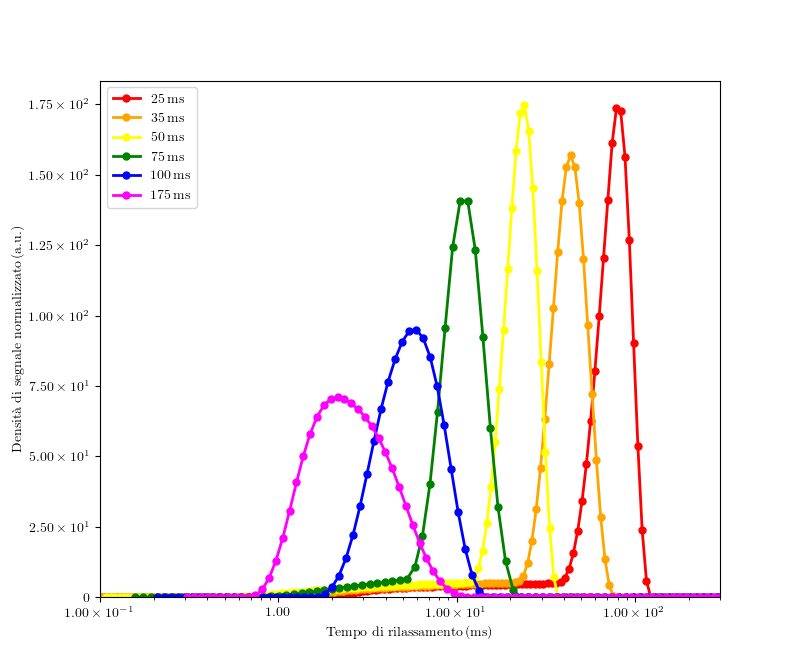
\includegraphics[scale=0.3]{Figure/H2O.png}
\caption{Distribuzioni dei tempi di rilassamento dell'acqua per ciascun $\tau$.}
\label{fig:D_h2o}
\end{figure}

\begin{figure}[ht]
\centering
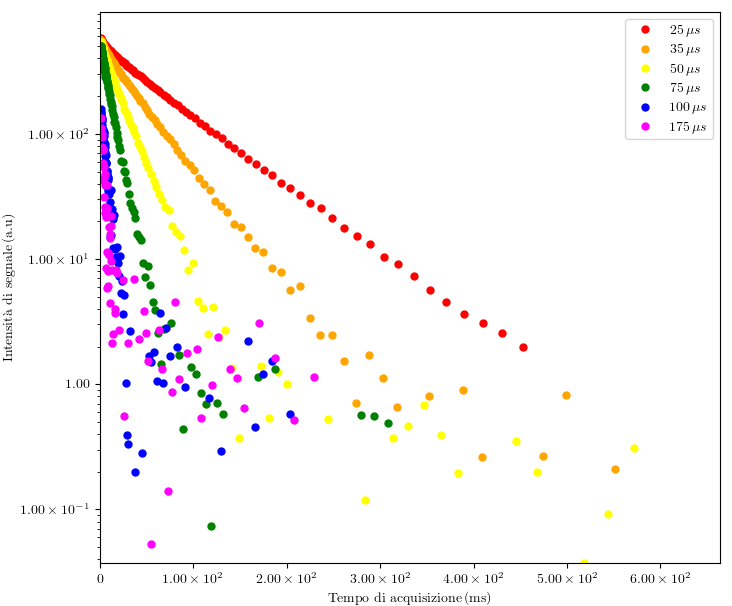
\includegraphics[scale=0.3]{Figure/H2O_SigTSig.png}
\caption{Intensità dei segnali dell'acqua per ciascun $\tau$.}
\label{fig:S_h2o}
\end{figure}

In seguito è stato calcolato analiticamente il coefficiente di autodiffusione a partire da una regressione lineare pesata eseguita sui dati di tabella \ref{tab:T_h2o}.
Il grafico seguente \ref{fig:Df_h2o} riporta l'andamento di tale fit.

\begin{figure}[ht]
\centering
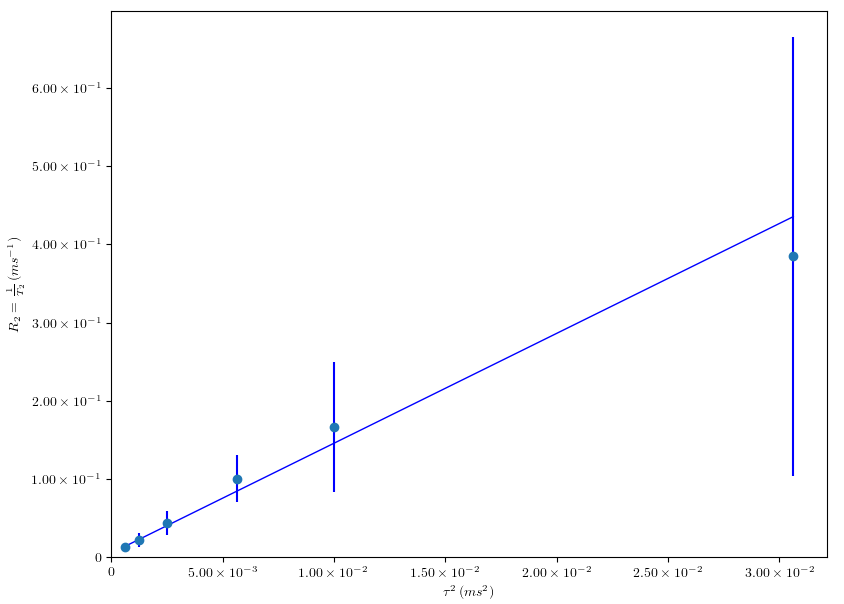
\includegraphics[scale=0.3]{Figure/H2O_calc.png}
\caption{Fit dei dati ottenuti per l'acqua.}
\label{fig:Df_h2o}
\end{figure}

Il risultato finale per il coefficiente di autodiffusione associato all'errore è riportato nella tabella seguente.

\begin{table}[ht]
    \begin{center}
    \begin{tabular}{c c c}
    \toprule
    	$D\,(\frac{{\mu}^2}{ms})$ & $\sigma\,(\frac{{\mu}^2}{ms})$ \\
    \midrule
    	2.04	&	0.16	\\
    \bottomrule
    \end{tabular}
    \caption{Coefficiente di autodiffusione dell'acqua con relativo errore.}
    \label{tab:Df_h2o}
    \end{center}
\end{table}


\subsection*{SOLTROL 130}

La seconda sostanza considerata è stata il soltrol 130.
Come per l'acqua, tramite il software UPENWin sono state delineate le distribuzioni dei tempi di rilassamento trasversali per $\tau$ (metà del tempo di eco) uguali a 20, 25, 30, 40, 50, 70, 90, 100 ${\mu}s$.

Sono riportate in tabella \ref{tab:T_s130} i tempi ottenuti con le relative incertezze, calcolate secondo lo stesso metodo applicato per l'acqua.

\begin{table}[ht]
    \begin{center}
    \begin{tabular}{c c c}
    \toprule
    	${\tau}\,({\mu}s)$ & $T\,(ms)$ & ${\sigma}\,(ms)$ \\
    \midrule
	 20 & 150 & 40 \\
	 25 & 120 & 30 \\
	 30 & 100 & 20 \\
	 40 & 67 & 16 \\
	 50 & 47 & 12 \\
	 70 & 27 & 6 \\
	 90 & 18 & 5 \\
	 100 & 15 & 4 \\
    \bottomrule
    \end{tabular}
    \caption{Tempi di rilassamento trasversale relativi ai diversi tempi $\tau$ per il soltrol 130.}
    \label{tab:T_s130}
    \end{center}
\end{table}

Sono stati poi descritti i grafici \ref{fig:D_s130} e \ref{fig:S_s130} che rappresentano le distribuzioni dei tempi di rilassamento e l'intensità dei segnali acquisiti per il soltrol 130 nella configurazione in cui UPENWin calcola il doppio dei punti d'inversione, ritenuta la più rappresentativa.

\begin{figure}[ht]
\centering
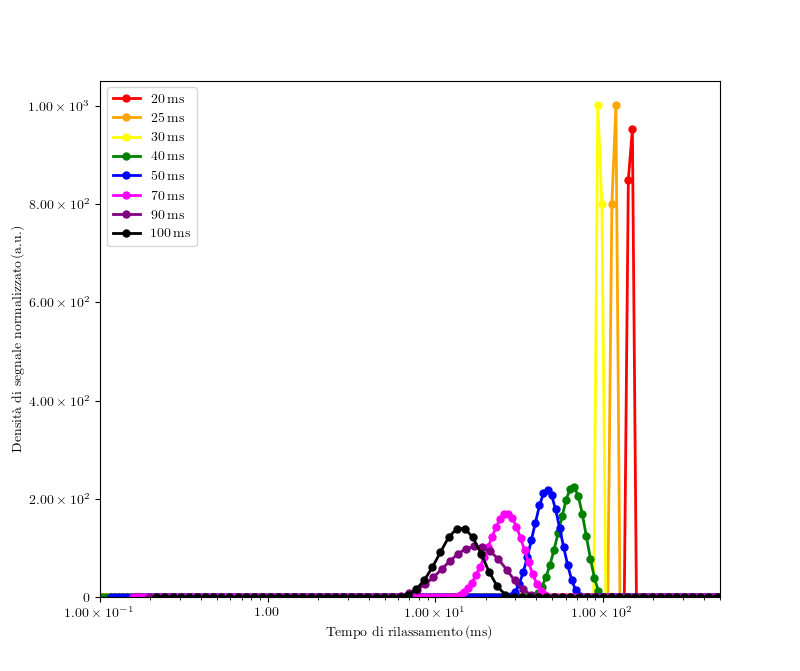
\includegraphics[scale=0.3]{Figure/SOLTROL130.png}
\caption{Distribuzioni dei tempi di rilassamento del soltrol 130 per ciascun $\tau$.}
\label{fig:D_s130}
\end{figure}

\begin{figure}[ht]
\centering
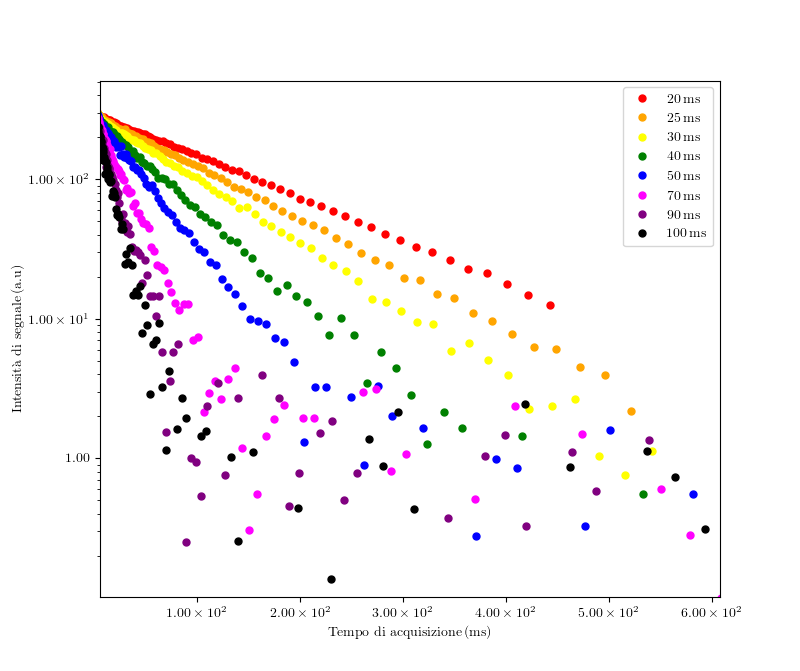
\includegraphics[scale=0.3]{Figure/SOLTROL130_SigTSig.png}
\caption{Intensità dei segnali del soltrol 130 per ciascun $\tau$.}
\label{fig:S_s130}
\end{figure}

\'E stato poi ottenuto il coefficiente di autodiffusione usando inizialmente una regressione lineare pesata eseguita sui dati di tabella \ref{tab:T_s130}, come proceduto per l'acqua.
Il grafico seguente \ref{fig:Df_s130} riporta l'andamento di tale fit.

\begin{figure}[ht]
\centering
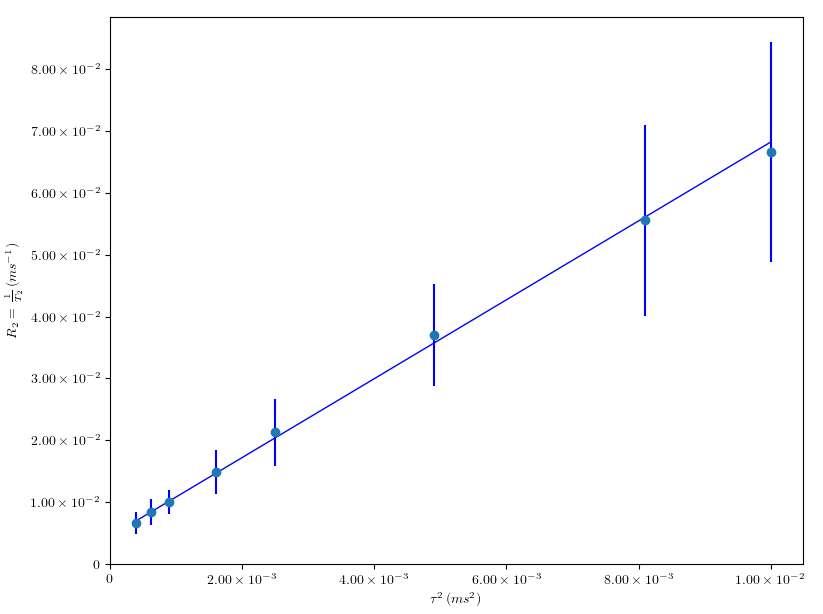
\includegraphics[scale=0.3]{Figure/SOLTROL130_calc.png}
\caption{Fit dei dati ottenuti per il soltrol 130.}
\label{fig:Df_s130}
\end{figure}

Il risultato finale per il coefficiente di autodiffusione del soltrol 130 assieme alla sua incertezza è riportato nella tabella seguente.

\begin{table}[h!]
    \begin{center}
    \begin{tabular}{c c c}
    \toprule
    	$D\,(\frac{{\mu}^2}{ms})$ & $\sigma\,(\frac{{\mu}^2}{ms})$ \\
    \midrule
    	0.927	&	0.015	\\
    \bottomrule
    \end{tabular}
    \caption{Coefficiente di autodiffusione del soltrol 130 con relativo errore.}
    \label{tab:Df_s130}
    \end{center}
\end{table}


\subsection*{SOLTROL 170}

L'ultima sostanza analizzatat è stata il soltrol 170.
Analogamente a come è stato eseguito per l'acqua e il soltrol 130, il software UPENWin è stato adoperato per descrivere le distribuzioni dei tempi di rilassamento trasversali per $\tau$ (metà del tempo di eco) pari a 25, 50, 75, 100, 125, 150 ${\mu}s$.

Nella tabella seguente \ref{tab:T_s130} sono riportati i tempi calcolati assieme all'errore associato, ricavati come citato in precedenza.

\begin{table}[ht]
    \begin{center}
    \begin{tabular}{c c c}
    \toprule
    	${\tau}\,({\mu}s)$ & $T\,(ms)$ & ${\sigma}\,(ms)$ \\
    \midrule
	 25 & 200 & 50 \\
	 50 & 100 & 30 \\
	 75 & 51 & 12 \\
	 100 & 33 & 7 \\
	 125 & 21 & 5 \\
	 150 & 14 & 3 \\
    \bottomrule
    \end{tabular}
    \caption{Tempi di rilassamento trasversale relativi ai diversi tempi $\tau$ per il soltrol 170.}
    \label{tab:T_s170}
    \end{center}
\end{table}

I grafici seguenti \ref{fig:D_s170} e \ref{fig:S_s170} mostrano le distribuzioni dei tempi di rilassamento e l'intensità dei segnali acquisiti per il soltrol 170 nella configurazione rappresentativa, in cui UPENWin calcola il doppio dei punti d'inversione.

\begin{figure}[ht]
\centering
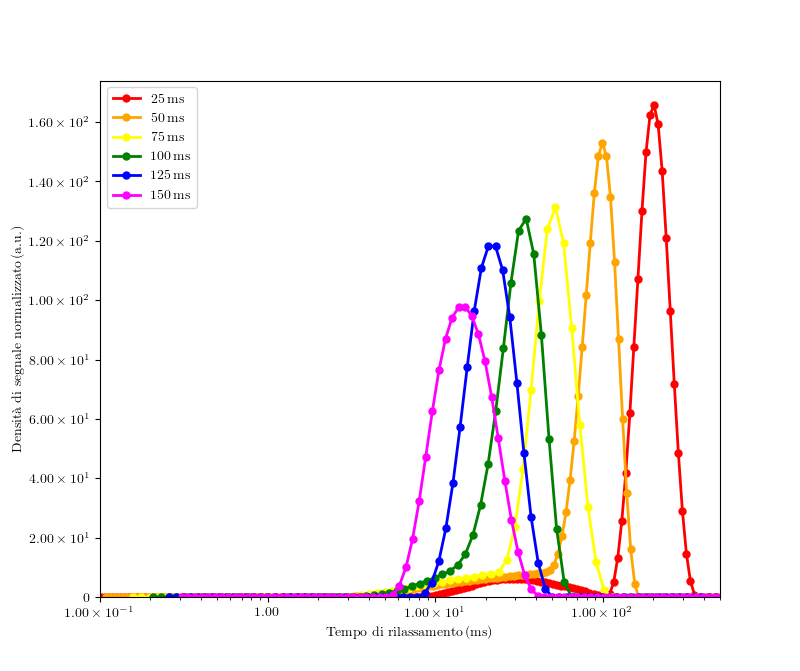
\includegraphics[scale=0.3]{Figure/SOLTROL170.png}
\caption{Distribuzioni dei tempi di rilassamento del soltrol 170 per ciascun $\tau$.}
\label{fig:D_s170}
\end{figure}

\begin{figure}[ht]
\centering
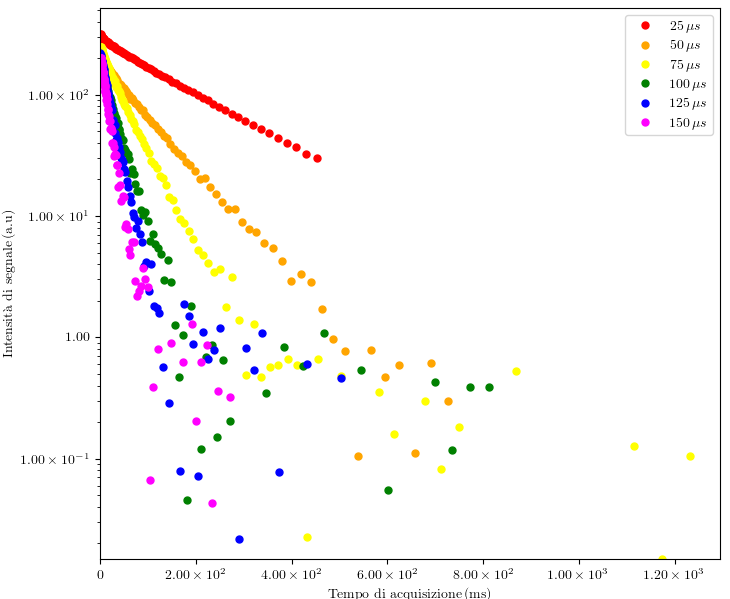
\includegraphics[scale=0.3]{Figure/SOLTROL170_SigTSig.png}
\caption{Intensità dei segnali del soltrol 170 per ciascun $\tau$.}
\label{fig:S_s170}
\end{figure}

Successivamente è stato ricavato il coefficiente di autodiffusione applicando una regressione lineare pesata sui dati di tabella \ref{tab:T_s170}, allo stesso modo che per l'acqua e il soltrol 130.
Il grafico \ref{fig:Df_s170} riporta l'andamento del fit.

\begin{figure}[ht]
\centering
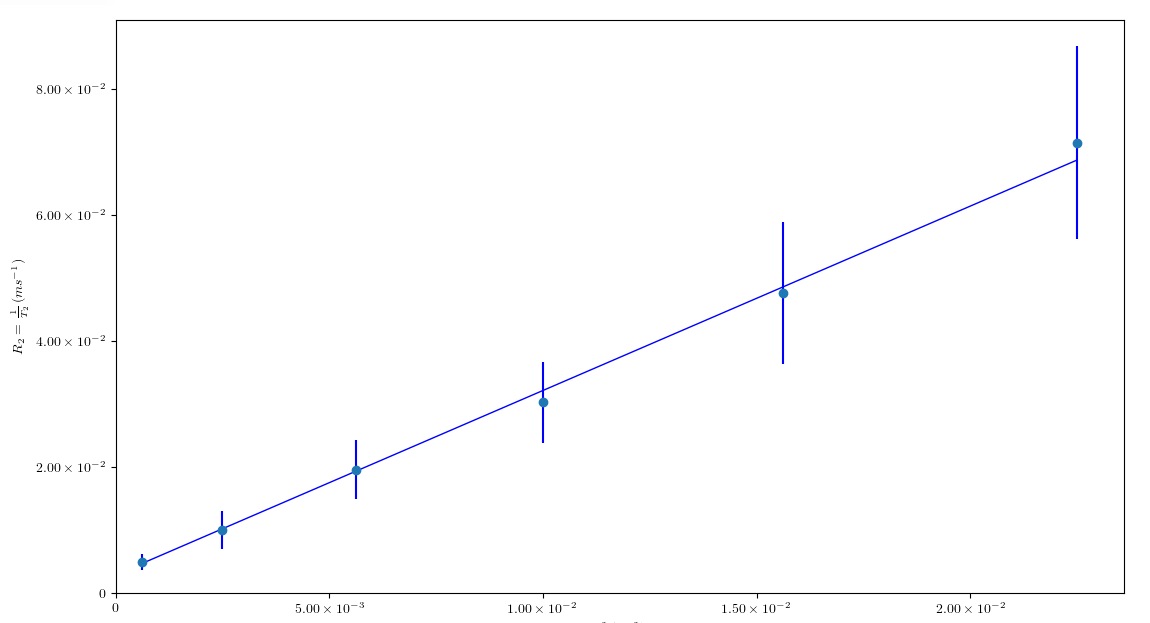
\includegraphics[scale=0.3]{Figure/SOLTROL170_calc.png}
\caption{Fit dei dati ottenuti per il SOLTROL 170.}
\label{fig:Df_s170}
\end{figure}

Il risultato finale per il coefficiente di autodiffusione del soltrol 170 affetto da errore è contenuto in tabella \ref{tab:T_s170}. 


\begin{table}[ht]
    \begin{center}
    \begin{tabular}{c c c}
    \toprule
    	$D\,(\frac{{\mu}^2}{ms})$ & $\sigma\,(\frac{{\mu}^2}{ms})$ \\
    \midrule
    	0.425	&	0.011	\\
    \bottomrule
    \end{tabular}
    \caption{Coefficiente di autodiffusione del soltrol 170 con relativo errore.}
    \label{tab:Df_s170}
    \end{center}
\end{table}






\section*{Conclusione}
I risultati esposti in precedenza hanno evidenziato come sia per l'albume che per il tuorlo siano presenti impurità.
Nel primo caso è plausibile che tale impurità sia presente solo in piccole dosi, vista la scarsa intensità del segnale; mentre nel secondo caso è supponibile che il tuorlo sia costituito da più composti.

Per dare un'ulteriore solidità a tale risultato si consideri il grafico \ref{fig:SigT_Sig}. 
Da questo tipo di illustrazione è possibile valutare quanto i campioni siano descritti da un andamento monoesponenziale e quindi siano costituiti da un solo componente.

Le curve relative ai tempi di rilassamento dell'albume descrivono un andamento lineare finchè il segnale non ha intensità pari a quella del rumore. 
Ciò implica che l'effetto più rilevante è dato dal singolo costituente dell'albume e l'effetto dato dall'impurità è trascurabile, confermando la leggera presenza ipotizzata precedentemente.

Riguardo al tuorlo invece è possibile notare che per entrambi i tempi di rilassamento si ha un andamento che approssima inizialmente una retta ma che rapidamente si inclina per formare una curva.
Ciò rafforza l'idea che il tuorlo non sia costituito da un solo composto ma da diversi.

\begin{figure}[h]
\centering
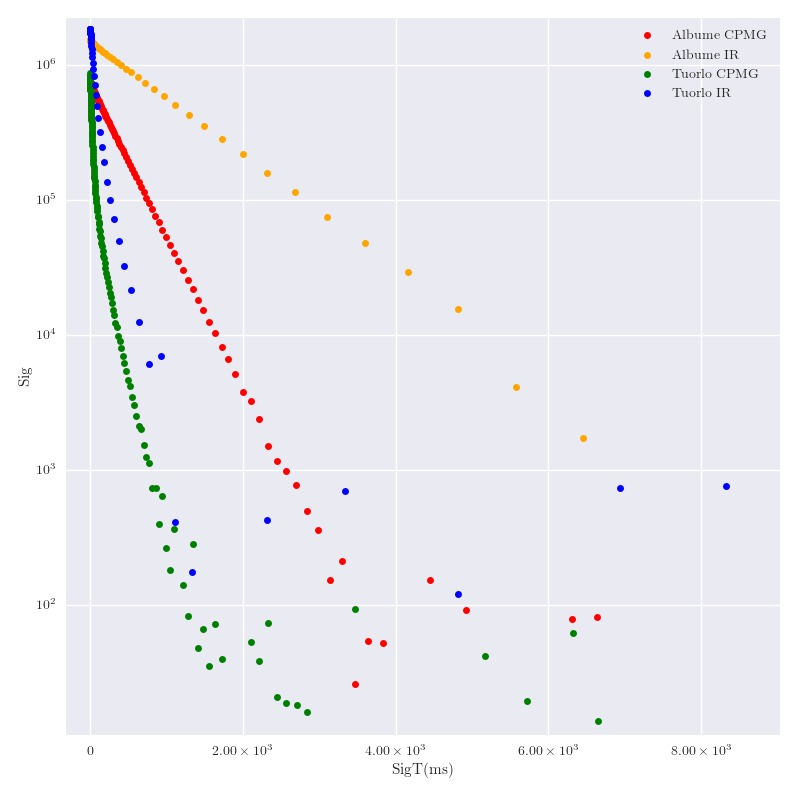
\includegraphics[scale=0.3]{SigT_Sig.jpeg}
\caption{Rappresentazione semilogaritmica della relazione tra l'intensità del segnale acquisito e il tempo di acquisizione.}
\label{fig:SigT_Sig}
\end{figure}


Oltre a valutare la composizione di albume e tuorlo, è possibile dedurre dai risultati della sezione precedente che il contrasto che si può ottenere tra immagini pesato in $T_1$ e $T_2$ è alto per entrambi i campioni.
Infatti, per ognuno dei due si hanno tempi di rilassamento $T_2$ molto inferiori a $T_1$.

Avendo ottenuto i valori di $T_1$ e $T_2$ per il tuorlo e per l'albume, è ora possibile sfruttare la formula seguente di MRI Spin-Echo con metodo spin warp per calcolare gli intervalli di $T_E$ e $T_R$ per ricavare immagini pesate.

${M_y}_{(T_R,T_E)} = M_0[1-e^{-\frac{T_R}{T_1}}(2e^{-\frac{T_{E/2}}{T_1}}-1)]e^{-\frac{T_E}{T_2}}$		\\
	
\'E stato tracciato il grafico tridimensionale \ref{3D} del contrasto in funzione di $T_E$ e $T_R$ appartenti al range $10-1000\,ms$, i cui valori indicano rispettivamente il limite strumentale e il valore massimo entro il quale è ragionevole ripetere la sequenza. 
Inoltre, sono stati tracciati i grafici \ref{} e \ref{} per ricavare gli intervalli di immagini pesate per $T_1$ e $T_2$.
Per pesare in $T_1$ è stato fissato il $T_E$ al minimo strumentale ed è stato ricercato l'intervallo rispetto a $T_R$; mentre per pesare in $T_2$ è stato fissato $T_R$ pari al massimo valore di ripetibilità ed è stato ricercato l'intervallo su $T_E$.

\begin{figure}[h]
\centering
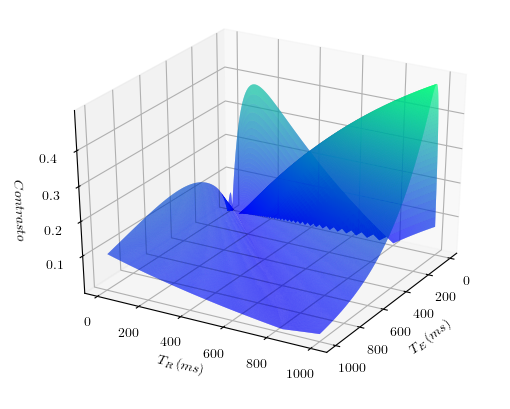
\includegraphics[scale=0.3]{3Dw.png}
\caption{Rappresentazione 3D del contrasto tra albume e tuorlo.}
\label{fig:3D}
\end{figure}

\begin{figure}[h]
\centering
\subfloat[][\emph{Andamento rispetto a $T_R$ per pesare in $T_1$.}]
	{\label{subfig:T1}
	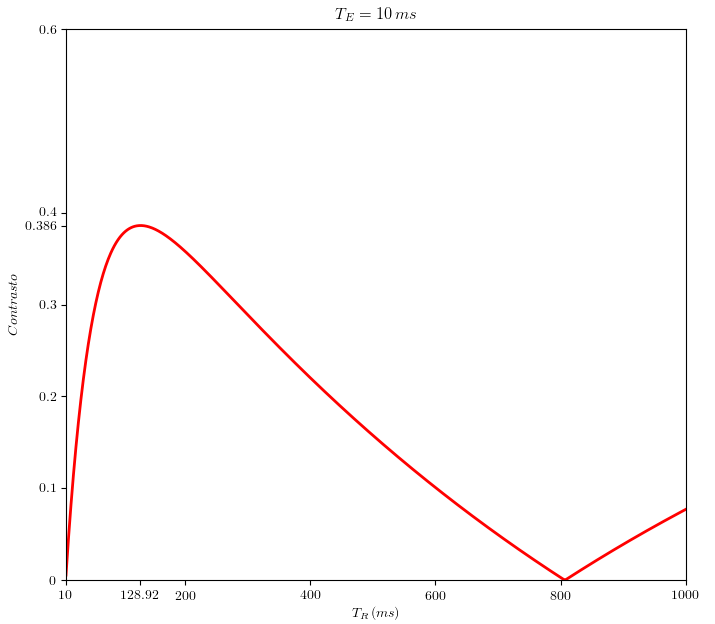
\includegraphics[scale=.18]{T1w.png}
	} \quad
\subfloat[][\emph{Andamento rispetto a $T_E$ per pesare in $T_R$.}]
	{\label{subfig:T2}
	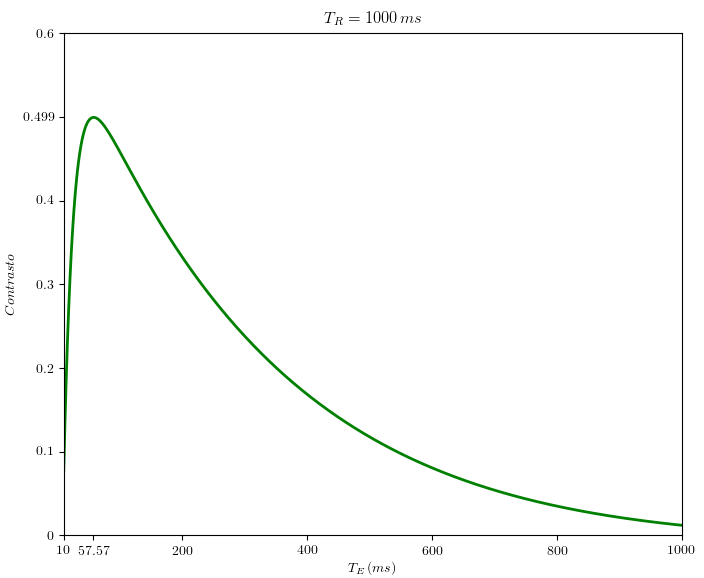
\includegraphics[width=.4\textwidth]{T2w.png}
	} \\
\caption{}
\label{fig:Contrasto}
\end{figure}


La tabella seguente contiene gli intervalli derivati approssimati al valore dell'intero più vicino.


\begin{table}[h]
	\centering
	\begin{tabular}{ccc}
	\toprule
		\textbf{Pesate in $T_1$} &	\textbf{Pesate in $T_2$}	\\
	\midrule
		$T_E = 10\,ms$			&		$T_E = 60\,ms$	 \\	
		$T_R = 130\,ms$			&		$T_R = 1000\,ms$ \\
	\bottomrule
	\end{tabular}
	\caption{Stime degli intervalli per $T_E$ e $T_R$ per generare immagini MRI pesate.}	
	\label{tab:Pesate}
\end{table}

\begin{thebibliography}{9}

\bibitem{UpenWIN}
  Bortolotti V., Brown R.J.S., Fantazzini P.,
  \textit{UpenWin Software},
  \url{http://software.dicam.unibo.it/upenwin%20},
  2012.

\bibitem{website}
 Hornak Joseph P.,
 \textit{The Basics of MRI},
 \url{https://www.cis.rit.edu/htbooks/mri/inside-i.htm},
 2016.

 \bibitem{dhawan2011medical}
 Dhawan Atam P.,
 \textit{Medical image analysis},
 2011.

\end{thebibliography}

\end{document}